\documentclass[10pt]{beamer}
% \documentclass[handout,10pt]{beamer}
\usepackage{my_style}
%%%%%%%%%%%%%%%%%%%%%%%%%%%%%%%%%%%%%%%%%%%%%%%%%%%%%%%%%%%%%%%%%%%%%%%%

\title[Math/CS 375]{Lecture 11 - B}
\subtitle{\S 5.1, 5.3 Newton-Cotes}

\begin{document}
\begin{frame}
  \titlepage
\end{frame}
%%%%%%%%%%%%%%%%%%%%%%%%%%%%%%%%%%%%%%%%%%%
\begin{frame}{Goals}
We will answer these questions:\\[3mm]
\begin{itemize}
    \item How accurate is Trapezoid method?
    \item What is Simpson's rule and how accurate is it?
    \item What are Newton-Cotes rules and how are they related to splines? 
\end{itemize}
\end{frame}

%%%%%%%%%%%%%%%%%%%%%%%%%%%%%%%%%%%%%%%%%%%
\sectionframe{Interpolation Review}
%%%%%%%%%%%%%%%%%%%%%%%%%%%%%%%%%%%%%%%%%%%



\begin{frame}{First-Degree Spline}

\define{First-Degree Spline }{
A function $S(x)$ is a \textbf{spline of degree 1} if it satisfies all of the following:
\begin{enumerate}
  \item The domain of $S(x)$ is an interval $[a,b]$
  \item $S(x)$ is continuous on $[a,b]$
  \item There is a partition $a=t_0<t_1<\dots<t_n=b$ such that $S(x)$ is
\emph{linear} on each subinterval $[t_i,t_{i+1}]$.
\end{enumerate}
}
\begin{center}
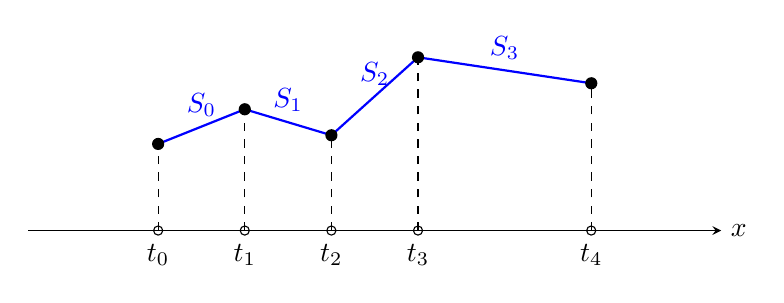
\begin{tikzpicture}[scale=1.1,>=stealth]
% Axis
\draw[->] (-1.5,0) -- (6.5,0) node[right] {$x$};

% Knot positions
\foreach \x/\label in {0/t_0,1/t_1,2/t_2,3/t_3,5/t_4} {
    \draw (\x,0) circle (1.5pt);
    \node[below] at (\x,-0.05) {$\label$};
}

% Points (ti, yi)
\coordinate (P0) at (0,1);
\coordinate (P1) at (1,1.4);
\coordinate (P2) at (2,1.1);
\coordinate (P3) at (3,2.0);
\coordinate (P4) at (5,1.7);

% Vertical dashed lines
\foreach \p in {P0,P1,P2,P3,P4} {
    \draw[dashed] (\p |- 0,0) -- (\p);
}

% Spline segments
\draw[thick,blue] (P0) -- (P1) node[midway,above] {$S_0$};
\draw[thick,blue] (P1) -- (P2) node[midway,above] {$S_1$};
\draw[thick,blue] (P2) -- (P3) node[midway,above] {$S_2$};
\draw[thick,blue] (P3) -- (P4) node[midway,above] {$S_3$};

% Data points
\foreach \p in {P0,P1,P2,P3,P4} {
    \fill (\p) circle (2pt);
}

\end{tikzpicture}
\end{center}
\end{frame}
%%%%%%%%%%%%%%%%%%%%%%%%%%%%%%%%%%%%%%%%%%%%%%%%%%%%%%%%%%%%%%%%%%%%%%%%



%%%%%%%%%%%%%%%%%%%%%%%%%%%%%%%%%%%%%%

\begin{frame}{Linear Approximation}
\begin{center}
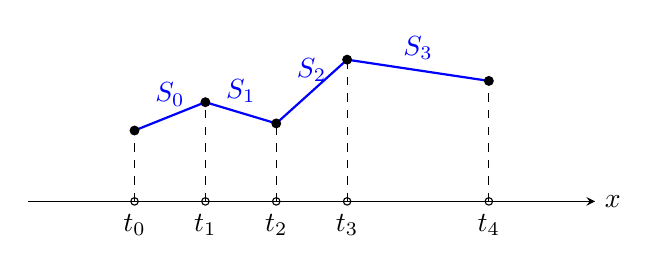
\begin{tikzpicture}[scale=0.9,>=stealth]
% Axis
\draw[->] (-1.5,0) -- (6.5,0) node[right] {$x$};

% Knot positions
\foreach \x/\label in {0/t_0,1/t_1,2/t_2,3/t_3,5/t_4} {
    \draw (\x,0) circle (1.5pt);
    \node[below] at (\x,-0.05) {$\label$};
}

% Points (ti, yi)
\coordinate (P0) at (0,1);
\coordinate (P1) at (1,1.4);
\coordinate (P2) at (2,1.1);
\coordinate (P3) at (3,2.0);
\coordinate (P4) at (5,1.7);

% Vertical dashed lines
\foreach \p in {P0,P1,P2,P3,P4} {
    \draw[dashed] (\p |- 0,0) -- (\p);
}

% Spline segments
\draw[thick,blue] (P0) -- (P1) node[midway,above] {$S_0$};
\draw[thick,blue] (P1) -- (P2) node[midway,above] {$S_1$};
\draw[thick,blue] (P2) -- (P3) node[midway,above] {$S_2$};
\draw[thick,blue] (P3) -- (P4) node[midway,above] {$S_3$};

% Data points
\foreach \p in {P0,P1,P2,P3,P4} {
    \fill (\p) circle (2pt);
}

\end{tikzpicture}
\end{center}
\begin{itemize}
    \item Each piece of the spline is a linear function 
    $$
        S_i(x) = a_i x + b_i
    $$
\end{itemize}

\end{frame}

%%%%%%%%%%%%%%%%%%%%%%%%%%%%%%%%%%%%%%
\begin{frame}{Approximating Functions}
\begin{center}
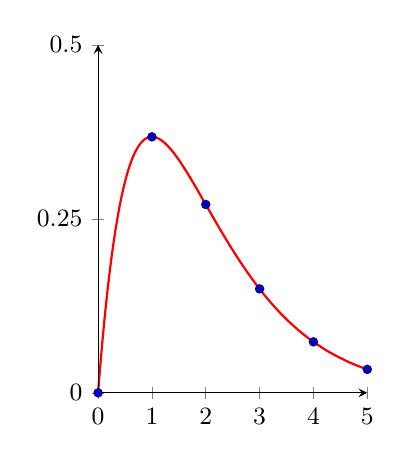
\begin{tikzpicture}
\begin{axis}[
    width=5cm,
    height=6cm,
    axis lines=left,
    xmin=0, xmax=5,
    ymin=0, ymax=0.5,
    domain=0:5,
    samples=300,
    xtick={0,1,...,5},
    ytick={0,0.25,...,0.5},
    tick label style={font=\small},
    xlabel={},
    ylabel={},
    axis on top,
    clip=false
]

% exact curve
\addplot[red, thick] {x*exp(-x)};


\addplot[
    only marks,
    mark=*,
    mark size=1.5pt,
    blue!70!black
] coordinates {
    (0,{0*exp(0)})
    (1,{1*exp(-1)})
    (2,{2*exp(-2)})
    (3,{3*exp(-3)})
    (4,{4*exp(-4)})
    (5,{5*exp(-5)})
};

\end{axis}
\end{tikzpicture}
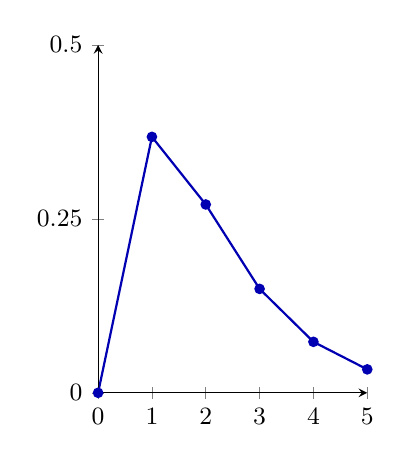
\begin{tikzpicture}
\begin{axis}[
    width=5cm,
    height=6cm,
    axis lines=left,
    xmin=0, xmax=5,
    ymin=0, ymax=0.5,
    domain=0:5,
    samples=300,
    xtick={0,1,...,5},
    ytick={0,0.25,...,0.5},
    tick label style={font=\small},
    xlabel={},
    ylabel={},
    axis on top,
    clip=false
]

% exact curve
% \addplot[red, thick] {x*exp(-x)};


\addplot[
    mark=*,
    mark size=1.5pt,
    blue!70!black,thick
] coordinates {
    (0,{0*exp(0)})
    (1,{1*exp(-1)})
    (2,{2*exp(-2)})
    (3,{3*exp(-3)})
    (4,{4*exp(-4)})
    (5,{5*exp(-5)})
};

\end{axis}
\end{tikzpicture}
\end{center}
\begin{itemize}
    \item A function can be sampled and approximated with a degree one spline
\end{itemize}
\end{frame}

%%%%%%%%%%%%%%%%%%%%%%%%%%%%%%%%%%


\begin{frame}{Interpolation Error}
\begin{center}

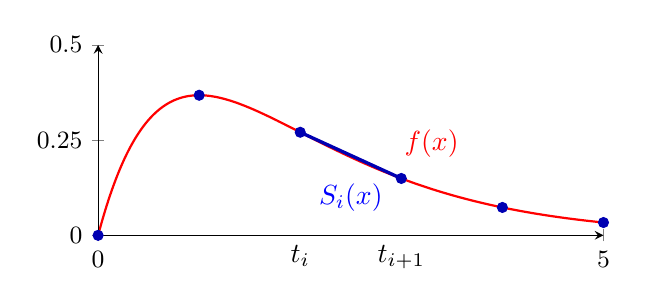
\begin{tikzpicture}
\begin{axis}[
    width=8cm,
    height=4cm,
    axis lines=left,
    xmin=0, xmax=5,
    ymin=0, ymax=0.5,
    domain=0:5,
    samples=300,
    xtick={0,5},
    ytick={0,0.25,...,0.5},
    tick label style={font=\small},
    xlabel={},
    ylabel={},
    axis on top,
    clip=false
]

% exact curve
\addplot[red, thick] {x*exp(-x)};

% nodes
\addplot[
    only marks,
    mark=*,
    mark size=1.8pt,
    blue!70!black
] coordinates {
    (0,{0})
    (1,{1*exp(-1)})
    (2,{2*exp(-2)})
    (3,{3*exp(-3)})
    (4,{4*exp(-4)})
    (5,{5*exp(-5)})
};

% spline segment from 2 to 3
\addplot[
    very thick,
    blue!70!black
] coordinates {
    (2,{2*exp(-2)})
    (3,{3*exp(-3)})
};

% label nodes t_i and t_{i+1}
\node[below] at (axis cs:2,0) {$t_i$};
\node[below] at (axis cs:3,0) {$t_{i+1}$};

% label spline
\node[blue] at (axis cs:2.5,0.1) {$S_i(x)$};

% label function
\node[red] at (axis cs:3.3,0.24) {$f(x)$};

\end{axis}
\end{tikzpicture}

\end{center}

\begin{block}{Degree One Spline Error}
We know the error on each spline piece
$$
e_i(x) = f(x)-S_i(x) = \frac{(x-t_i)(x-t_{i+1})}{2} f''(c)
$$
\end{block}
\end{frame}

%%%%%%%%%%%%%%%%%%%%%%%%%%%%%%%%%%%%%%%%%%%
\sectionframe{Trapezoid Error Analysis}
%%%%%%%%%%%%%%%%%%%%%%%%%%%%%%%%%%%%%%%%%%%
\begin{frame}{Truth about Trapezoid Method}

\begin{block}{}
    Here's the truth about trapezoid method
\end{block}
Trapezoid method is actually just:
\onslide<2>{

\begin{enumerate}
    \item Approximating $f(x)$ with a degree 1 spline $S(x)$,
    \item Then integrating the spline $\int S(x)\,dx$
\end{enumerate}
\begin{center}
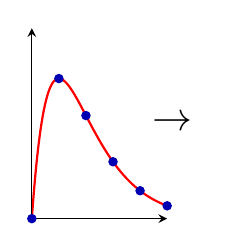
\begin{tikzpicture}
\begin{axis}[
    width=3.3cm,
    height=4cm,
    axis lines=left,
    xmin=0, xmax=5,
    ymin=0, ymax=0.5,
    domain=0:5,
    samples=300,
    xtick={0,1,...,5},
    ytick={0,0.25,...,0.5},
    xticklabels=\empty,
    yticklabels=\empty,
    xlabel={},
    ylabel={},
    axis on top,
    clip=false,
    ticks=none
]
% exact curve
\addplot[red, thick] {x*exp(-x)};
\addplot[
    only marks,
    mark=*,
    mark size=1.5pt,
    blue!70!black
] coordinates {
    (0,{0*exp(0)})
    (1,{1*exp(-1)})
    (2,{2*exp(-2)})
    (3,{3*exp(-3)})
    (4,{4*exp(-4)})
    (5,{5*exp(-5)})
};
\node at (5.2,0.25) {\Large $\rightarrow$};
\end{axis}
\end{tikzpicture}
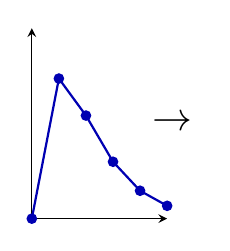
\begin{tikzpicture}
\begin{axis}[
    width=3.3cm,
    height=4cm,
    axis lines=left,
    xmin=0, xmax=5,
    ymin=0, ymax=0.5,
    domain=0:5,
    samples=300,
    xtick={0,1,...,5},
    ytick={0,0.25,...,0.5},
    xticklabels=\empty,
    yticklabels=\empty,
    xlabel={},
    ylabel={},
    axis on top,
    clip=false,
    ticks=none
]

% exact curve
% \addplot[red, thick] {x*exp(-x)};
\addplot[
    mark=*,
    mark size=1.5pt,
    blue!70!black,thick
] coordinates {
    (0,{0*exp(0)})
    (1,{1*exp(-1)})
    (2,{2*exp(-2)})
    (3,{3*exp(-3)})
    (4,{4*exp(-4)})
    (5,{5*exp(-5)})
};
\node at (5.2,0.25) {\Large $\rightarrow$};
\end{axis}
\end{tikzpicture}
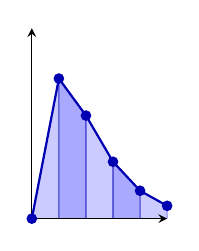
\begin{tikzpicture}
\begin{axis}[
    width=3.3cm,
    height=4cm,
    axis lines=left,
    xmin=0, xmax=5,
    ymin=0, ymax=0.5,
    domain=0:5,
    samples=300,
    xtick={0,1,...,5},
    ytick={0,0.25,...,0.5},
    xticklabels=\empty,
    yticklabels=\empty,
    xlabel={},
    ylabel={},
    axis on top,
    clip=false,
    ticks=none
]
% composite trapezoids, h = 1
\addplot[draw=blue!70!black, fill=blue!45, opacity=0.45]
coordinates {(0,0) (0,{0*exp(0)}) (1,{1*exp(-1)}) (1,0)};

\addplot[draw=blue!70!black, fill=blue!75, opacity=0.45]
coordinates {(1,0) (1,{1*exp(-1)}) (2,{2*exp(-2)}) (2,0)};

\addplot[draw=blue!70!black, fill=blue!45, opacity=0.45]
coordinates {(2,0) (2,{2*exp(-2)}) (3,{3*exp(-3)}) (3,0)};

\addplot[draw=blue!70!black, fill=blue!75, opacity=0.45]
coordinates {(3,0) (3,{3*exp(-3)}) (4,{4*exp(-4)}) (4,0)};

\addplot[draw=blue!70!black, fill=blue!45, opacity=0.45]
coordinates {(4,0) (4,{4*exp(-4)}) (5,{5*exp(-5)}) (5,0)};

% nodes on the curve
\addplot[
    thick,
    mark=*,
    mark size=1.5pt,
    blue!70!black
] coordinates {
    (0,{0*exp(0)})
    (1,{1*exp(-1)})
    (2,{2*exp(-2)})
    (3,{3*exp(-3)})
    (4,{4*exp(-4)})
    (5,{5*exp(-5)})
};

\end{axis}
\end{tikzpicture}
\end{center}
}
\end{frame}
%%%%%%%%%%%%%%%%%%%%%%%%%%%%%%%%%%%%%%%%%%%

\begin{frame}{Why does that matter?}

{
\question{
        Why is it useful to think of it  as the integral of a degree 1 spline?
}
}
    \vspace{3mm}
    
    \begin{itemize}
        \item We know the interpolation error 
            $$e_1(x) =  f(x) - p_1 (x) = \frac{(x-x_0)(x-x_1)}{2} f''(c)$$
            

        \begin{center}
        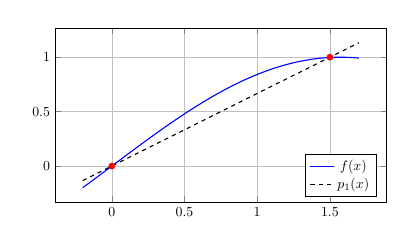
\begin{tikzpicture}[scale=0.5]
        \begin{axis}[
            width=10cm, height=6cm,
            xlabel={}, ylabel={},
            grid=major, 
            thick,
            domain=0:2,
            samples=100,
            legend pos=south east
        ]
        
            % Define the function f(x) = sin(x)
            \addplot[color=blue, thick, domain=-0.2:1.7] {sin(deg(x))};
            \addlegendentry{$f(x)$};
        
            % Plot the linear interpolant (straight line between x_0=0 and x_1=pi/2)
            \addplot[color=black, dashed, thick] coordinates {(-0.2,-0.133) (1.7,1.133)};
            \addlegendentry{$p_1(x)$};
        
            % Mark points x_0 = 0 and x_1 = pi/2 on the curve
            \addplot[mark=*, only marks, color=red] coordinates {(0, 0) (1.5, 1)};
        \end{axis}
        \end{tikzpicture}
        \end{center}
    \end{itemize}
    \keyidea{
    We may use the interpolation error formula.
    }
\end{frame}
%%%%%%%%%%%%%%%%%%%%%%%%%%%%%%%%%%%%%%%%%%%
\begin{frame}{Trapezoid Error}{Illustration}

    \cols{
    \begin{center}
        
    \begin{tikzpicture}[scale=1.0]
    \begin{axis}[
        width=6cm, height=4cm,
        xlabel={}, ylabel={},
        grid=major, 
        thick,
        domain=0:2,
        samples=50,
    ]
        % Define and plot the function f(x) = sin(x)
        \addplot[name path=func, color=blue, thick, domain=-0.2:1.7] {sin(deg(x))};
        % \addlegendentry{$f(x) = \sin(x)$};
    
        % Define the x-axis path from x=0 to x=1.5
        \addplot[name path=xaxis, draw=none, domain=0:1.5] {0};
    
        % Shade the area under f(x) between x=0 and x=1.5
        \addplot [
            fill=blue!20,    % Fill color
            fill opacity=0.3, % Adjust opacity here
            draw=none
        ] fill between [
            of=func and xaxis,
            soft clip={domain=0:1.5},
        ];
        % Plot the linear interpolant (straight line between x=0 and x=1.5)
        \addplot[color=black, dashed, thick] coordinates {(-0.2,-0.133) (1.7,1.133)};
        % \addlegendentry{$p_1(x)$};
    
        % Mark points x=0 and x=1.5 on the curve
        \addplot[mark=*, only marks, color=red] coordinates {(0, 0) (1.5, 1)};
    \end{axis}
    \end{tikzpicture}\\
    $I = \int_a^b f(x)\,dx$
    \end{center}
    
    }{
    \begin{center}
        
    \begin{tikzpicture}[scale=1.0]
    \begin{axis}[
        width=6cm, height=4cm,
        xlabel={}, ylabel={},
        grid=major, 
        thick,
        domain=0:2,
        samples=50,
    ]
    
        % Define and plot the function f(x) = sin(x)
        \addplot[name path=func, color=blue, thick, domain=-0.2:1.7] {sin(deg(x))};
        % \addlegendentry{$f(x) = \sin(x)$};
    
        % Define the x-axis path from x=0 to x=1.5
        \addplot[name path=xaxis, draw=none, domain=0:1.5] {0};
    
        % Shade the area under the linear interpolant to illustrate the trapezoidal method
        \addplot [
            fill=blue!20,       % Fill color
            fill opacity=0.5,    % Adjust opacity here
            draw=none
        ] coordinates {(0,0) (1.5,1) (1.5,0) (0,0)};
    
        % Plot the linear interpolant (straight line between x=0 and x=1.5)
        \addplot[color=black, dashed, thick] coordinates {(-0.2,-0.133) (1.7,1.133)};
        % \addlegendentry{$p_1(x)$};
    
        % Mark points x=0 and x=1.5 on the curve
        \addplot[mark=*, only marks, color=red] coordinates {(0, 0) (1.5, 1)};
    \end{axis}
    \end{tikzpicture}
     $T = \int_a^b p_1(x)\,dx$\\
    \end{center}
    }
\vspace{5mm}
   \begin{block}{Trapezoid Error}
        $$E = I - T = \int_a^b f(x)\,dx - \int_a^b p_1(x)\,dx $$
   \end{block}

\end{frame}


%%%%%%%%%%%%%%%%%%%%%%%%%%%%%%%%%%%%%%%%%%%
\begin{frame}{Accuracy for Basic Trapezoid}{Part 1}
\begin{itemize}
    \item Substitute the interpolation error 
            $$f(x) - p_1 (x) = \frac{(x-x_0)(x-x_1)}{2} f''(c)$$
    \item into the integration error equation
        \begin{align*}
          E &= \int_a^b f(x)\,dx - \int_a^b p_1(x) \,dx =  \int_a^b(f(x) - p_1(x))\,dx \\
            &= \frac{1}{2}\int_a^b f''(c) (x-a)(x-b) \,dx \,\quad  ( \text{ note} (x-a)(x-b) \leq 0 \text{ in } [a,b])\\
            &= \frac{f''(c)}{2}\int_a^b  (x-a)(x-b) \,dx \,\quad (\text{use MVT to extract }f''(c))         
            \end{align*}
\end{itemize}
\end{frame}

%%%%%%%%%%%%%%%%%%%%%%%%%%%%%%%%%%%%%%%%%%%
\begin{frame}{Accuracy for Basic Trapezoid}{Part 2}
\begin{itemize}
    \item Integration by parts, $u=(x-b)$ and $dv=(x-a)\,dx$
        \begin{align*}
          E &= \frac{f''(c)}{2}\int_a^b  (x-a)(x-b) \,dx \\
           &= \frac{f''(c)}{2}\left(\frac12(x-a)^2(x-b)\Bigg|_a^b-\frac12\int_a^b  (x-a)^2 \,dx\right) \\  
          &=\frac{f''(c)}{2}\left(-\frac{1}{6}(b-a)^3\right)\\ 
          &=-\frac{(b-a)^3 f''(c)}{12}
        \end{align*}
\end{itemize}
    \question{This is the error for basic trapezoid. What about the composite trapezoid?}
\end{frame}


%%%%%%%%%%%%%%%%%%%%%%%%%%%%%%%%%%%%%%%%%%%
\begin{frame}{Accuracy for Composite Trapezoid}{Part 1}
\begin{itemize}
    \item Composite Trapezoid is just basic trapezoid $n$ times
        \begin{equation*}
          \int_a^b f(x)\,dx \approx T_{\text{comp}} = \sum_{i=0}^{n-1}T_i
        \end{equation*}
    \item The error in each interval $[x_i,x_{i+1}]$ is
        \begin{equation*}
        E_i = \int_{x_i}^{x_{i+1}}f(x)\,dx-T_i= -\frac{(x_{i+1}-x_i)^3 f''(c)}{12} =-\frac{h^3 f''(c_i)}{12}
        \end{equation*}
    \item The \textbf{total error} can be derived by adding up each error
        \begin{align*}
        E_{\textrm{comp}} &= \sum_{i=0}^{n-1} E_i = \sum_{i=0}^{n-1}  -\frac{h^3 f''(c_i)}{12}\\ 
        \end{align*}
\end{itemize}
\end{frame}
%%%%%%%%%%%%%%%%%%%%%%%%%%%%%%%%%%%%%%%%%%%
\begin{frame}[shrink]{Accuracy for Composite Trapezoid}{Part 2}
\begin{itemize}
    \item By the continuity of $f''$, we can argue an average value of $f(c_i)$
        $$
        f''(c)=\sum_{i=0}^{n-1} \frac{f''(c_i)}{n}
        $$
    \item Now we can manipulate the total error by multiplying by $\frac{n}{n}$
        \begin{align*}
        E_{\textrm{comp}} & = \sum_{i=0}^{n-1}  -\frac{h^3 f''(c_i)}{12} \frac{n}{n}\\
        &= -n \frac{h^3}{12} \sum_{i=0}^{n-1}  \frac{f''(c_i)}{n}\\ 
         & = \frac{-nh^3}{12} f''(c)
        \end{align*}
    \item Finally, use the fact that $n=\frac{b-a}{h}$
        \begin{align*}
        E_{\textrm{comp}} &= \frac{-nh^3}{12} f''(c)  = -\frac{(b-a) h^2 f''(c)}{12}
        \end{align*}
\end{itemize}
\end{frame}
%%%%%%%%%%%%%%%%%%%%%%%%%%%%%%%%%%%%%%%%%%%
\begin{frame}{Trapezoid Error}
\begin{block}{Basic Trapezoidal Rule Error}
    $$E = -\frac{(b-a)^3 f''(c)}{12}$$
\end{block}
\begin{block}{Composite Trapezoidal Rule Error}
    $$E_{\textrm{comp}} = -\frac{(b-a) h^2 f''(c)}{12} = \mO(h^2) $$
\end{block}
\begin{itemize}
    \item $n$ = number of subintervals, $h$ = width of trapezoids
    \item As $n\rightarrow\infty $, the error goes to zero quadratically
\end{itemize}

    \question{How can we utilize the Composite Error Formula?}
\end{frame}
%%%%%%%%%%%%%%%%%%%%%%%%%%%%%%%%%%%%%%%%%%%
\begin{frame}[shrink]{Using the Error Theorem}
\begin{example}
What value of $n$ will ensure the composite Trapezoid rule is accurate to $\epsilon = 10^{-6}$ for $\int_0^1 e^{-x^2}\,dx$?
\end{example}
\begin{itemize}
    \item Set up the inequality $E < \epsilon $ 
        \begin{equation*}
        \frac{(b-a) h^2 f''(c)}{12} \leq 10^{-6}
        \end{equation*}
    \item Find worst case scenario for $f''(c)$
        \begin{align*}
          f(x) &= e^{-x^2}\\
          f'(x) &=-2xe^{-x^2}\\
          f''(x) &=-2e^{-x^2}+4x^2e^{-x^2} = 2e^{-x^2}(2x^2-1)
        \end{align*}
        On the interval $[0,1]$, we have the estimate $f''(x)\le 2.$ 
    \item Finally we solve for $n$
        \begin{equation*}
        E = \frac{(b-a) 2 h^2}{12} = \frac{(b-a)^3}{6n^2} = \frac{1}{6n^2}  \leq 10^{-6}
        \end{equation*}
        \begin{equation*}
         n^{2} \ge  10^{6}/6   \Rightarrow  n \ge 10^{3}/\sqrt{6} \approx 408.2
        \end{equation*}

\end{itemize}
\end{frame}
%%%%%%%%%%%%%%%%%%%%%%%%%%%%%%%%%%%%%%%%%%%
\begin{frame}{Using the Error Theorem}

\begin{itemize}
    \item This is a theoretical error bound 
        $$E_{\textrm{comp}} = -\frac{(b-a) h^2 f''(c)}{12}$$

    \item For the specific example $\int_0^1 e^{-x^2}\,dx$, we found 
    $$
        E < 10^{-6} \quad\text{ when }\quad n>408 
    $$
    \item In practice, we may need fewer trapezoids than $408$

    \keyidea{
    The error formula allows us to estimate the number of trapezoids needed to approximate an integral up to any tolerance level.
    }
\end{itemize}
    
\end{frame}

%%%%%%%%%%%%%%%%%%%%%%%%%%%%%%%%%%%%%%%%%%%
\begin{frame}{How do we improve Trapezoid?}
    \begin{itemize}
    \item Riemann Sum = integrate degree ZERO spline \bigskip
    \item Composite Trapezoid = integrate degree ONE spline \bigskip
    \begin{alertblock}{}
        How do you improve?
    \end{alertblock}\bigskip
    \item<2-> Integrate a degree \emph{TWO} spline 
\end{itemize}
\end{frame}
%%%%%%%%%%%%%%%%%%%%%%%%%%%%%%%%%%%%%%%%%%%
\sectionframe{Simpson's Rule}
%%%%%%%%%%%%%%%%%%%%%%%%%%%%%%%%%%%%%%%%%%%
\begin{frame}{Basic Simpson}{The Idea}
\begin{center}
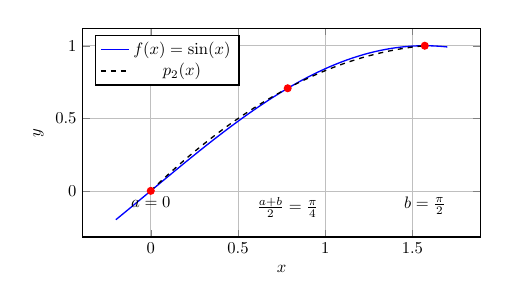
\begin{tikzpicture}[scale=0.6]
\begin{axis}[
    width=10cm, height=6cm,
    xlabel={$x$}, ylabel={$y$},
    grid=major, 
    thick,
    domain=0:2,
    samples=100,
    legend pos=north west,
]

    % Define the function f(x) = sin(x)
    \addplot[color=blue, thick, domain=-0.2:1.7] {sin(deg(x))};
    \addlegendentry{$f(x) = \sin(x)$};

    % Plot the quadratic interpolant through x_0 = 0, x_1 = pi/3, x_2 = pi/2
    % Quadratic interpolant formula for sin(x) through these points
    % Plot the correct quadratic interpolant through x_0 = 0, x_1 = pi/3, x_2 = pi/2
    \addplot[color=black, dashed, thick, domain=0:1.5708] 
    {-(8*sqrt(2)*x^2)/pi^2 + (8*x^2)/pi^2 + (4*sqrt(2)*x)/pi - (2*x)/pi};
    \addlegendentry{$p_2(x)$};

    % Mark points x_0 = 0, x_1 = pi/3, and x_2 = pi/2 on the curve
    \addplot[mark=*, only marks, color=red] 
    coordinates {(0, 0) (0.785, 0.707) (1.5708, 1)};
    
    % Annotate x_0, x_1, and x_2
    \node at (axis cs:0,0) [below] {$a = 0$};
    \node at (axis cs:0.785,0.0) [below] {$\frac{a+b}{2} = \frac{\pi}{4}$};
    \node at (axis cs:1.5708,0.0) [below] {$b = \frac{\pi}{2}$};

\end{axis}
\end{tikzpicture}
\end{center}

    Steps:
  \begin{enumerate}
      \item Approximate $f(x)$ with a quadratic $p_2(x)$
    \item Approximate $\int f(x) \,dx \approx \int p_2(x)\,dx$
  \end{enumerate}
    \keyidea{
    Simpson's rule says integrate the quadratic interpolation $p_2(x)$ rather than the actual function.
    }
\end{frame}
%%%%%%%%%%%%%%%%%%%%%%%%%%%%%%%%%%%%%%%%%%%
%%%%%%%%%%%%%%%%%%%%%%%%%%%%%%%%%%%%%%%%%%%
\begin{frame}[shrink]{Basic Simpson Derivation}{Part 1}
The goal is to approximate Consider $\int_{a}^{b} f(x)\,dx$\\[3mm]
  \begin{itemize}
  \item Let $h=\frac{b-a}{2}$. Then partition $P =\{a,a+h,b=a+2h\}$ 
  \item To simplify things, consider $\int_{0}^{2h} f(x)\,dx$ so partition $P =\{0,h,2h\}$\smallskip
  \item Use Newton Divided difference to find  $p_2(x)$:
    \begin{align*}
      f(x) & \approx p_2(x)\\
          &= a_0 + a_1 x + a_2 x(x-h)
           % & = f(0) + \frac{f(h)-f(0)}{h} x + \frac{f(2h)-2f(h)+f(0)}{2h^2} x (x-h)
    \end{align*}
    \item The coefficients are 
    \begin{align*}
        a_0 &= f[0] = f(0) \\ 
        a_1 &= f[0,h] = \frac{f(h) - f(0)}{h}\\
        a_2 &= f[0,h,2h] = \frac{\frac{f(2h)-f(h)}{h}-\frac{f(h)-f(0)}{h}}{2h} = \frac{f(2h)-2f(h)+f(0)}{2h^2}
    \end{align*}
  % \item Integrate $\int_{0}^{2h} p_2(x)\,dx$ to get the basic Simpson's formula
  % \begin{align*}
  % \int_{0}^{2h} f(x)\,dx &\approx \int_{0}^{2h} p_2(x)\,dx\\
  %                        &= \frac{h}{3}\left[f(0) + 4f(h) + f(2h)\right]
  % \end{align*}
\end{itemize}
\end{frame}
%%%%%%%%%%%%%%%%%%%%%%%%%%%%%%%%%%%%%%%%%%%
\begin{frame}[shrink]{Basic Simpson Derivation}{Part 2}
  \begin{itemize}
  \item The Newton interpolation is 
    \begin{align*}
      f(x) & \approx p_2(x) = f(0) + \frac{f(h)-f(0)}{h} x + \frac{f(2h)-2f(h)+f(0)}{2h^2} x (x-h)
    \end{align*}
  \item Now integrate $\int_{0}^{2h} p_2(x)\,dx$ to get the basic Simpson's formula
  \begin{align*}
  \int_{0}^{2h} p_2(x) \,dx &=  \int_{0}^{2h} f(0) + \frac{f(h)-f(0)}{h} x + \frac{f(2h)-2f(h)+f(0)}{2h^2} x (x-h)\,dx\\
                            &= 2h f(0) + \frac{f(h)-f(0)}{h} (2h^2) + \frac{f(2h)-2f(h)+f(0)}{2h^2} \frac{2h^3}{3} \\
                            &= f(0)\left[ 2h - 2h +\frac{h}{3}\right] + f(h)\left[ 2h -\frac{2h}{3} \right]+f(2h)\left[\frac{h}{3}\right]\\
                         &= \frac{h}{3}\left[f(0) + 4f(h) + f(2h)\right]\\
                         &= \frac{2h}{6}\left[f(0) + 4f(h) + f(2h)\right]\\
  \end{align*}
\end{itemize}
\end{frame}
%%%%%%%%%%%%%%%%%%%%%%%%%%%%%%%%%%%%%%%%%%%
\begin{frame}{Basic Simpson}
\begin{block}{Basic Simpson's Rule}
  \begin{equation*}
  \int_{a}^{b} f(x)\,dx \approx \frac{b-a}{6}\left[f(a) + 4f\left(\frac{a+b}{2}\right) + f(b)\right]
  \end{equation*}
\end{block}
\begin{center}
  \pgfimage[height=5.25cm]{./figs/basicsimpson1}
\end{center}
\end{frame}

\begin{frame}{Ratio $1:4:1$}

\begin{itemize}
    \item Simpson's formula acts as a weighted average
    \begin{equation*}
  \int_{a}^{b} f(x)\,dx \approx \frac{b-a}{6}\left[f(a) + 4f\left(\frac{a+b}{2}\right) + f(b)\right]
  \end{equation*}

  \item It has the form
  $$
    I \approx (b-a) \left(\frac{1f(x_{left})+4f(x_{mid})+1f(x_{right})}{6}\right)
  $$

  \item Therefore, Simpson's is a $1:4:1$ weighted average of the values of $f(x)$
\end{itemize}
    
\end{frame}

%%%%%%%%%%%%%%%%%%%%%%%%%%%%%%%%%%%%%%%%%%%

\begin{frame}{Hand Calculation}

\begin{example}
    Approximate the following integral using the basic Simpson's rule:
    \[
        \int_0^4 x\,dx.
    \]
\end{example}

\begin{itemize}
    \item The endpoints and midpoint are $0$, $2$, and $4$.
    \item Apply Simpson's rule:
    \[
    \begin{aligned}
        \int_a^b f(x)\,dx
        &\approx \frac{b-a}{6}
        \left[f(a)+4f\left(\frac{a+b}{2}\right)+f(b)\right]\\[2mm]
        \int_0^4 x\,dx
        &\approx \frac{4-0}{6}\left[0+4(2)+4\right]\\
        &= \frac{4}{6}(12)=8.
    \end{aligned}
    \]
\end{itemize}



\end{frame}

%%%%%%%%%%%%%%%%%%%%%%%%%%%%%%%%%%%%%%%%%%%
\sectionframe{Composite Rule}
%%%%%%%%%%%%%%%%%%%%%%%%%%%%%%%%%%%%%%%%%%%

\begin{frame}[shrink]{Using Simpson's Rule Twice for one Interval}

\question{
How would you use the basic Simpson's rule twice under one interval $[a,b]?$
}


\begin{itemize}
    \item You would have to divide $[a,b]$ into 4 even subintervals with nodes 
        $$ \{  x_0 = a,\; x_1, x_2, x_3,\; x_4=b\}$$
    \item The first Simpson's rule approximates integral over $\{x_0, x_1, x_2\}$ 
         $$I_0 = \int_{x_0}^{x_2} S_0(x) \,dx = \frac{x_2-x_0}{6} \left[f(x_0) + 4f(x_1) + f(x_2) \right] $$
    \item The second Simpson's rule approximates integral over $\{x_2, x_3, x_4\}$ 
         $$I_1 = \int_{x_2}^{x_4} S_1(x) \,dx = \frac{x_4-x_2}{6} \left[f(x_2) + 4f(x_3) + f(x_4) \right] $$
    \item When we combine the two...
        \begin{align*}
        I_0 + I_1 &=\frac{x_2-x_0}{6} \left[f(x_0) + 4f(x_1) + f(x_2) \right] + \frac{x_4-x_2}{6} \left[f(x_2) + 4f(x_3) + f(x_4) \right]\\
                  &=\frac{h}{3} \left[f(x_0) + 4f(x_1) + \textcolor{red}{{f(x_2)}} \right] + \frac{h}{3} \left[\textcolor{red}{f(x_2)} + 4f(x_3) + f(x_4) \right]\\
                  &=\frac{h}{3} \left[f(x_0) + 4f(x_1) + \textcolor{red}{2f(x_2)} + 4f(x_3) + f(x_4) \right]\\
        \end{align*}

\end{itemize}



\end{frame}

%%%%%%%%%%%%%%%%%%%%%%%%%%%%%%%%%%%%%%%%%%%
\begin{frame}{Composite Simpson}
\begin{itemize}
    \item Divide $[a,b]$ into $n$ subintervals, $n$ must be an \emph{even number}

\item Apply basic Simpson's Rule over groups of 2 subintervals $[x_{2i},x_{2i+2}]$ 
  \begin{align*}
  \int_{a}^{b} f(x)\,dx & \approx \sum_{i=0}^{n/2-1} \int_{x_{2i}}^{x_{2i+2}} f(x)\,dx\\
                        & = \sum_{i=0}^{n/2-1} \frac{2h}{6}\left[f(x_{2i}) + 4f(x_{2i+1}) + f(x_{2i+2})\right]\\
                        & = \frac{h}{3}[f(x_{0}) + \textcolor{blue}{4f(x_1)} + \textcolor{red}{2f(x_2)} + \textcolor{blue}{4f(x_3)} + \textcolor{red}{2f(x_4)}+ \cdots \\
                        & \quad \quad \textcolor{blue}{4f(x_{n-1})} +f(x_{n})]
  \end{align*}
  \item Inner coefficients alternate between 4 and 2.
\end{itemize}
\end{frame}
%%%%%%%%%%%%%%%%%%%%%%%%%%%%%%%%%%%%%%%%%%%
\begin{frame}{Composite Simpson}{Formula}
\begin{block}{Composite Simpson's Rule}
  \begin{equation*}
  \int_{a}^{b} f(x)\,dx \approx \frac{h}{3}\left[f(a) + 4 \sum_{i=1}^{n/2} f(a+(2i-1)h) + 2\sum_{i=1}^{n/2 - 1}f(a+2ih) + f(b) \right]
  \end{equation*}
\end{block}

\begin{block}{Alternate Formula}
    \begin{equation*}
    \int_{a}^{b} f(x)\,dx \approx \frac{h}{3}\left[f(x_0) + 4 \left(\sum_{i \in [1,n-1]}^{i\;\text{is odd}} f(x_i)\right) + 2\left(\sum_{i \in [2,n-1]}^{i\;\text{is even}}f(x_i)\right) + f(x_n) \right]
    \end{equation*}
\begin{itemize}
\item The odd nodes $2i-1$ have weight 4 
\item The even nodes $2i$ have weight 2
\item The endpoints have weight 1
\end{itemize}
\end{block}

\end{frame}
%%%%%%%%%%%%%%%%%%%%%%%%%%%%%%%%%%%%%%%%%%%

\begin{frame}[fragile]{Composite Simpson}{The method}

\method{Uniform Composite Simpson's Method}
{Function $f(x)$, interval $[a,b]$, even number of subintervals $n$}{Approximation to $\int_a^b f(x) \,dx$}{
Integrate a degree 2 spline of $f(x)$.
}
    \begin{equation*}
    \int_{a}^{b} f(x)\,dx \approx \frac{h}{3}\left[f(x_0) + 4 \left(\sum_{i \in [1,n-1]}^{i\;\text{is odd}} f(x_i)\right) + 2\left(\sum_{i \in [2,n-1]}^{i\;\text{is even}}f(x_i)\right) + f(x_n) \right]
    \end{equation*}
    $$n\; \text{is even},\quad h = \frac{b-a}{n}$$
\end{frame}

%%%%%%%%%%%%%%%%%%%%%%%%%%%%%%%%%%%%%%%%%%%
\sectionframe{Simpson Error Analysis}
%%%%%%%%%%%%%%%%%%%%%%%%%%%%%%%%%%%%%%%%%%%
\begin{frame}{Composite Simpson}{Numerical Test}

\question{How does Composite Simpson performs in terms of $h$?}
\begin{itemize}
    \item Composite Trapezoid has order 2 convergence: 
        $$E_{\text{trap}}= \mO(h^2)$$

    \item We can guess that 
        $$E_{\text{simp}}= \mO(h^p)$$
        
    \item Run the experiment \texttt{simpson\_int\_test.m}
        \vfill
    \item<2> We get $p=4$?
\end{itemize}

\end{frame}
%%%%%%%%%%%%%%%%%%%%%%%%%%%%%%%%%%%%%%%%%%%%%%%

\begin{frame}{Analysis is Needed}

\begin{itemize}
    \item Consider the integral
        $$
            \int_a^b f(x)\,dx 
        $$
    \item Let $h=(b-a)/2$ so that 
        $$
            a=a,\quad \frac{a+b}{2} = a+h,\quad b = a+2h
        $$
    \item Then the Simpson approximation is 
        $$
            \int_a^{a+2h} f(x)\,dx \approx \frac{h}{3}\left[f(a)+4f(a+h)+f(a+2h)\right]
        $$
    \end{itemize}

    \begin{block}{Goal}
        We will study the error for Simpson's by Taylor expanding $f(x)$ around $x=a$.
    \end{block}

    
\end{frame}

%%%%%%%%%%%%%%%%%%%%%%%%%%%%%%%%%%%%%%%%%%%%%%%

\begin{frame}{Basic Simpson Error}{Part 1}
\begin{itemize}
    \item First, Taylor expand around $a$
        \begin{align*}
        f(a) & = f\\
        f(a+h) & = f + hf' + \frac{1}{2!}h^2 f'' + \frac{1}{3!}h^3 f''' + \frac{1}{4!}h^4 f^{(4)} + \frac{1}{5!}h^5 f^{(5)} + \dots\\
        f(a+2h) & = f + 2hf' + 2h^2 f'' + \frac{4}{3}h^3 f''' + \frac{2}{3}h^4 f^{(4)} + \frac{4}{15}h^5 f^{(5)} + \dots\\
        \end{align*}
    \item This gives
        \begin{equation*}
        \frac{h}{3}\left[f(a)+4f(a+h)+f(a+2h)\right] = 2hf +2h^2f' + \frac{4}{3}h^3f''+\frac{2}{3}h^4f'''+\frac{5}{18}h^5f^{(4)}
        \end{equation*}
\end{itemize}

\end{frame}
%%%%%%%%%%%%%%%%%%%%%%%%%
\begin{frame}{Basic Simpson Error}{Part 2}
\begin{itemize}
    \item Consider the antiderivative of $f(x)$:
        \[
        F(x) = \int_a^x f(t) \, dt
        \]
    \item Taylor series of $F$:
        \[
        F(a+2h) = F(a) + 2h F'(a) + 2h^2 F''(a) + \frac{4}{3}h^3F'''(a) + \frac{2}{3} h^4 F^{(4)} +\frac{4}{15}h^5 F^{(5)} + \cdots
        \]
    \item Noting that $F(a+2h) = \int_{a}^{b=a+2h}f(x)\,dx$, $F(a) = 0, F' = f, F'' = f'$ and so on,
        \begin{equation*}
        \int_{a}^{b=a+2h}f(x)\,dx = 2hf +2h^2f' + \frac{4}{3}h^3f''+\frac{2}{3}h^4f'''+\frac{4}{15}h^5f^{(4)} + \cdots
        \end{equation*}
% \begin{block}{Basic Simpson's Error}
% \begin{equation*}
% -\frac{1}{90}\left(\frac{b-a}{2}\right)^5 f^{(4)}(\xi)
% \end{equation*}
% \end{block}
\end{itemize}
\end{frame}
%%%%%%%%%%%%%%%%%%%%%%%%%%%%%%%%%%%%%%%%%%%
\begin{frame}{Basic Simpson Error}{Part 3}
\begin{itemize}
    \item The true value is 
        \begin{equation*}
        \int_{a}^{b=a+2h}f(x)\,dx = 2hf +2h^2f' + \frac{4}{3}h^3f''+\frac{2}{3}h^4f'''+\frac{4}{15}h^5f^{(4)} + \cdots
        \end{equation*}
    \item The approximation is
        \begin{equation*}
        \frac{h}{3}\left[f(a)+4f(a+h)+f(a+2h)\right] = 2hf +2h^2f' + \frac{4}{3}h^3f''+\frac{2}{3}h^4f'''+\frac{5}{18}h^5f^{(4)}
        \end{equation*}
    \item Thus, the error (their difference) is
    \begin{block}{Basic Simpson's Error}
    \begin{equation*}
    -\frac{1}{90}\left(\frac{b-a}{2}\right)^5 f^{(4)}(\xi)
    \end{equation*}
    \end{block}
\end{itemize}
\end{frame}
%%%%%%%%%%%%%%%%%%%%%%%%%%%%%%%%%%%%%%%%%%%
\begin{frame}{Why is composite Simpson $\mO(h^4)$?}
\begin{itemize}
    \item Error for one interval using basic Simpson's Rule:
        \begin{equation*}
        -\frac{1}{90}\left(\frac{b-a}{2}\right)^5 f^{(4)}(\xi)
        \end{equation*}
    \item Over $n/2$ subintervals $[x_{2i},x_{2i+2}]$, the error adds up to
\begin{align*}
err & =  \sum_{i=0}^{n/2-1} -\frac{1}{90}\left(\frac{x_{2i+2}-x_{2i}}{2}\right)^5 f^{(4)}(\xi_i)
      = -\frac{1}{90}  \sum_{i=0}^{n/2-1} \left(\frac{2h}{2}\right)^5 f^{(4)}(\xi_i)\\
    & = -\frac{1}{90}  \frac{n}{2}h^5 f^{(4)}(\xi)
      = -\frac{1}{180} \frac{(b-a)}{h}h^5 f^{(4)}(\xi)\\
    & = -\frac{b-a}{180} h^4 f^{(4)}(\xi)
\end{align*}
\vspace{-0.5cm}

\begin{block}{Composite Simpson's Rule Error}
\begin{equation*}
  -\frac{b-a}{180}h^4 f^{(4)}(\xi)
\end{equation*}
\end{block}
We ``gain'' two orders over Trapezoid -- got lucky!
\end{itemize}
\end{frame}
%%%%%%%%%%%%%%%%%%%%%%%%%%%%%%%%%%%%%%%%%%%

\begin{frame}{Summary}
Notice the pattern in our integration methods:



\begin{table}[h]
    \centering
    \begin{tabular}{lcc}
        \hline
        Method      & Description  & Accuracy\\
        \hline
        Left/Right Riemann & \parbox{5cm}{Approximate $f(x)\approx p_0(x)$\\  and integrate} & $\mO(h)$ \\
        Trapezoid   & \parbox{5cm}{Approximate $f(x) \approx p_1(x)$\\  and integrate} & $\mO(h^2)$\\
        Simpson     & \parbox{5cm}{Approximate $f(x) \approx p_2(x)$\\  and integrate} & $\mO(h^4)$\\
        \hline
    \end{tabular}
    % \caption{Integration Methods}
    \label{tab:integration_methods}
\end{table}
\bigskip 

Trapezoid and Simpson's both belong to a more general class of algorithms.
%\begin{block}{Degree of Precision} % according to Atkinson
%  If the integration rule has zero error when integrating any polynomial of
%degree $\leq r$
%\smallskip
%
%and
%\smallskip
%
%If the error is nonzero for some polynomial of degree $r+1$,
%
%and
%\smallskip
%
%then, the rule has \emph{degree of precision} equal to $r$.
%\end{block}
\end{frame}
%%%%%%%%%%%%%%%%%%%%%%%%%%%%%%%%%%%%%%%%%%%
\sectionframe{Newton-Cotes Formulas}
%%%%%%%%%%%%%%%%%%%%%%%%%%%%%%%%%%%%%%%%%%%
\begin{frame}{Going Further}
    \begin{table}[h]
    \centering
    \begin{tabular}{lcc}
        \hline
        Method      & Description  & Accuracy\\
        \hline
        Left/Right Riemann & $\int f(x)\approx \int p_0(x)$ & $\mO(h)$ \\
        Trapezoid   & $\int f(x) \approx \int p_1(x)$ & $\mO(h^2)$\\
        Simpson     & $\int f(x) \approx \int p_2(x)$ & $\mO(h^4)$\\
        \hline
    \end{tabular}
\end{table}
\bigskip 
\question{What's stopping us from going further: $\int p_3(x)$, $\int p_4(x)$, ...?}
\end{frame}

%%%%%%%%%%%%%%%%%%%%%%%%%%%%%%%%%%%%%%%%%%%
\begin{frame}{Newton-Cotes}

    \method{Newton-Cotes}
    {$f(x)$, interval $[a,b]$}
    {Approximation to $\int_a^bf(x)\,dx$}
    {Integrate the $n^{th}$ degree interpolation $\int_a^bf(x)\,dx \approx \int_a^b p_n(x)\,dx$}
    \vfill
    Properties: 
    \begin{itemize}
        \item The nodes $x_i$ are equally spaced out
        \item Have the form $ \int_a^b f(x)\, dx \approx \sum_{i=1}^n w_i f(x_i) $
        \item If $f(x)$ is an $n^{th}$ degree polynomial, then error is \textbf{zero}
    \end{itemize}

\end{frame}

%%%%%%%%%%%%%%%%%%%%%%%%%%%%%%%%%%%%%%%%%%%
%%%%%%%%%%%%%%%%%%%%%%%%%%%%%%%%%%%%%%%%%%%
% \begin{frame}
% \frametitle{Deriving Newton-Cotes Formulas}
%     Take an examples, say $n=4$: 
%     \begin{itemize}
%         \item All Newton-Cotes formulas have the form $ \int_a^b f(x)\, dx \approx \sum_{i=1}^n w_i f(x_i) $
%         \item If $f(x)$ is an $n^{th}$ degree polynomial, then error is \textbf{zero}
%     \end{itemize}

% \end{frame}

%%%%%%%%%%%%%%%%%%%%%%%%%%%%%%%%%%%%%%%%%%%
%%%%%%%%%%%%%%%%%%%%%%%%%%%%%%%%%%%%%%%%%%%
\begin{frame}
\frametitle{First Four Newton-Cotes Formulas}

   \textbf{Basic Newton-Cotes rules:}
   \begin{tabular}{l c l}
   name & $n$ & formula \\\hline
   Trapezoid       & 1 & $\frac{(b-a)}{2}\left[f(a) + f(b)\right]$\\[5pt]
   Simpson's $1/3$ & 2 & $\frac{(b-a)}{6}\left[f(a) + 4f(\frac{a+b}{2}) + f(b)\right]$\\[5pt]
   Simpson's $3/8$ & 3 & $\frac{(b-a)}{8}\left[f(a) + 3f(a+h) + 3f(b-h) + f(b)\right]$\\[5pt]
   Boole's         & 4 & $\frac{(b-a)}{90}\left[7f(a) + 32f(a+h) + 12f(\frac{a+b}{2}) + 32f(b-h)+7f(b)\right]$\\[5pt]
   \end{tabular}
   \smallskip

   \textbf{Error bounds for composite Newton-Cotes:}
   \begin{tabular}{l l l l}
   name & $n$ & error & $h$\\\hline
   Trapezoid       & 1 & $-\frac{(b-a)h^2}{12}f''(\xi)$ & $h=b-a$\\[5pt]
   Simpson's $1/3$ & 2 & $-\frac{(b-a)h^4}{180}f^{(4)}(\xi)$ & $h=(b-a)/2$\\[5pt]
   Simpson's $3/8$ & 3 & $-\frac{(b-a)h^4}{180}f^{(4)}(\xi)$ & $h=(b-a)/3$\\[5pt]
   Boole's         & 4 & $-\frac{2(b-a)h^6}{945}f^{(6)}(\xi)$ & $h=(b-a)/4$\\[5pt]
   \end{tabular}

\end{frame}
%%%%%%%%%%%%%%%%%%%%%%%%%%%%%%%%%%%%%%%%%%%
\begin{frame}{Newton-Cotes Error}

   \textbf{Error bounds for composite Newton-Cotes:}
   \begin{tabular}{l l l l}
   name & $n$ & error & $h$\\\hline
   Trapezoid       & 1 & $-\frac{(b-a)h^2}{12}f''(\xi)$ & $h=b-a$\\[5pt]
   Simpson's $1/3$ & 2 & $-\frac{(b-a)h^4}{180}f^{(4)}(\xi)$ & $h=(b-a)/2$\\[5pt]
   Simpson's $3/8$ & 3 & $-\frac{(b-a)h^4}{180}f^{(4)}(\xi)$ & $h=(b-a)/3$\\[5pt]
   Boole's         & 4 & $-\frac{2(b-a)h^6}{945}f^{(6)}(\xi)$ & $h=(b-a)/4$\\[5pt]
   \end{tabular}
   \vspace{5mm}
   \begin{itemize}
       \item Notice that Simpson's $1/3$ and Simpson's $3/8$ are both $\mO(h^4)$
       \item There is \emph{no} advantage going from degree 2 spline to degree 3 spline
   \end{itemize}

\end{frame}
%%%%%%%%%%%%%%%%%%%%%%%%%%%%%%%%%%%%%%%%%%%
\begin{frame}{Pattern to the Formulas}

   \textbf{Basic Newton-Cotes rules:}
   \begin{tabular}{l c l}
   name & $n$ & formula \\\hline
   Trapezoid       & 1 & $\frac{(b-a)}{2}\left[f(a) + f(b)\right]$\\[5pt]
   Simpson's $1/3$ & 2 & $\frac{(b-a)}{6}\left[f(a) + 4f(\frac{a+b}{2}) + f(b)\right]$\\[5pt]
   Simpson's $3/8$ & 3 & $\frac{(b-a)}{8}\left[f(a) + 3f(a+h) + 3f(b-h) + f(b)\right]$\\[5pt]
   Boole's         & 4 & $\frac{(b-a)}{90}\left[7f(a) + 32f(a+h) + 12f(\frac{a+b}{2}) + 32f(b-h)+7f(b)\right]$\\[5pt]
   \end{tabular}
   \smallskip
   
\begin{itemize}
    \item There is a pattern to all of the formulas 
    \item Let $a=x_0$, $b=x_n$, $h=\frac{b-a}{n}$, and $x_i = x_0 + ih $
    \item All of the formulas have the form 
        $$\sum_{i=0}^n  w_i  \, f(x_i)$$
\end{itemize}
\end{frame}
%%%%%%%%%%%%%%%%%%%%%%%%%%%%%%%%%%%%%%%%%%%
\begin{frame}{Remarks}
    \begin{itemize}
        \item There is a reference book for many Newton-Cotes formulas\\[4mm] 
        \item There are also ``Open" Newton-Cotes rules that do not use nodes at endpoints
            \begin{itemize}
                \item Midpoint rule is an example, composite midpoint is $\mO(h^2)$\\[4mm]
            \end{itemize}
        \item All formulas have a simple form making them easy to implement
            $$\sum_{i=0}^n  w_i  \, f(x_i)$$
        \item More preferable to do a composite Newton-Cotes with smaller $n$
            \begin{itemize}
                \item Two Composite Simpson's rule $>$ One Basic Boole's rule \\[4mm] 
            \end{itemize}
        \item \emph{Used to be} the most commonly used type of numerical integration
            \begin{itemize}
                \item We will learn Gaussian quadratures next
            \end{itemize}
    \end{itemize}
\end{frame}


\end{document}
